\documentclass[
11pt, % The default document font size, options: 10pt, 11pt, 12pt
codirector, % Uncomment to add a codirector to the title page
]{charter} 




% El títulos de la memoria, se usa en la carátula y se puede usar el cualquier lugar del documento con el comando \ttitle
\titulo{Firmware de dispositivo de adquisición de señales neurofisiológicas} 

% Nombre del posgrado, se usa en la carátula y se puede usar el cualquier lugar del documento con el comando \degreename
\posgrado{Carrera de Especialización en Sistemas Embebidos} 
%\posgrado{Carrera de Especialización en Internet de las Cosas} 
%\posgrado{Carrera de Especialización en Intelegencia Artificial}
%\posgrado{Maestría en Sistemas Embebidos} 
%\posgrado{Maestría en Internet de las cosas}

% Tu nombre, se puede usar el cualquier lugar del documento con el comando \authorname
\autor{Leandro Arrieta} 

% El nombre del director y co-director, se puede usar el cualquier lugar del documento con el comando \supname y \cosupname y \pertesupname y \pertecosupname
\director{Diego Coulombie}
\pertenenciaDirector{UNLaM} 
% FIXME:NO IMPLEMENTADO EL CODIRECTOR ni su pertenencia
\codirector{Ariel Gentile} % para que aparezca en la portada se debe descomentar la opción codirector en el documentclass
\pertenenciaCoDirector{Advantek}

% Nombre del cliente, quien va a aprobar los resultados del proyecto, se puede usar con el comando \clientename y \empclientename
\cliente{\supname}
\empresaCliente{UNLaM}

% Nombre y pertenencia de los jurados, se pueden usar el cualquier lugar del documento con el comando \jurunoname, \jurdosname y \jurtresname y \perteunoname, \pertedosname y \pertetresname.
\juradoUno{Nombre y Apellido (1)}
\pertenenciaJurUno{pertenencia (1)} 
\juradoDos{Nombre y Apellido (2)}
\pertenenciaJurDos{pertenencia (2)}
\juradoTres{Nombre y Apellido (3)}
\pertenenciaJurTres{pertenencia (3)}
 
\fechaINICIO{24 de junio de 2021}		%Fecha de inicio de la cursada de GdP \fechaInicioName
\fechaFINALPlan{19 de agosto de 2021} 	%Fecha de final de cursada de GdP
\fechaFINALTrabajo{15 de mayo de 2022}	%Fecha de defensa pública del trabajo final


\begin{document}

\maketitle
\thispagestyle{empty}
\pagebreak


\thispagestyle{empty}
{\setlength{\parskip}{0pt}
\tableofcontents{}
}
\pagebreak


\section*{Registros de cambios}
\label{sec:registro}


\begin{table}[ht]
\label{tab:registro}
\centering
\begin{tabularx}{\linewidth}{@{}|c|X|c|@{}}
\hline
\rowcolor[HTML]{C0C0C0} 
Revisión & \multicolumn{1}{c|}{\cellcolor[HTML]{C0C0C0}Detalles de los cambios realizados} & Fecha      \\ \hline
0      & Creación del documento                              & 01/07/2021 \\ \hline
1.0      & Se completa hasta la sección 5 inclusive          & 06/07/2021 \\ \hline
2.0      & Se agregan supuestos en la sección 5 \newline
		   Se completa hasta la sección 9 inclusive				 & 13/07/2021 \\ \hline
3.0      & Se agregan requerimientos de documentación \newline
		   Se completa hasta el punto 12 inclusive               & 26/07/2021 \\ \hline
4.0      &  Se agrega un item en la sección 4 \newline
			Se agrega un item en la sección 5 \newline
            Se completa el plan	                                 & 02/08/2021 \\ \hline
\end{tabularx}
\end{table}

\pagebreak



\section*{Acta de constitución del proyecto}
\label{sec:acta}

\begin{flushright}
Buenos Aires, \fechaInicioName
\end{flushright}

\vspace{2cm}

Por medio de la presente se acuerda con el Ing. \authorname\hspace{1px} que su Trabajo Final de la \degreename\hspace{1px} se titulará ``\ttitle'', consistirá esencialmente en el desarrollo y la implementación del firmware del dispositivo perteneciente al proyecto de investigación ''C2-ING-066 Herramientas de uso comunitario para el desarrollo de la industria de Tecnología Neurofisiológica", y tendrá un presupuesto preliminar estimado de 630 hs de trabajo, con fecha de inicio \fechaInicioName\hspace{1px} y fecha de presentación pública \fechaFinalName.

Se adjunta a esta acta la planificación inicial.

\vfill

% Esta parte se construye sola con la información que hayan cargado en el preámbulo del documento y no debe modificarla
\begin{table}[ht]
\centering
\begin{tabular}{ccc}
\begin{tabular}[c]{@{}c@{}}Ariel Lutenberg \\ Director posgrado FIUBA\end{tabular} & \hspace{2cm} & \begin{tabular}[c]{@{}c@{}}\clientename \\ \empclientename \end{tabular} \vspace{2.5cm} \\ 
%\multicolumn{3}{c}{\begin{tabular}[c]{@{}c@{}} \supname \\ Director del Trabajo Final\end{tabular}} \vspace{2.5cm} \\
%\begin{tabular}[c]{@{}c@{}}\jurunoname \\ Jurado del Trabajo Final\end{tabular}     &  & \begin{tabular}[c]{@{}c@{}}\jurdosname\\ Jurado del Trabajo Final\end{tabular}  \vspace{2.5cm}  \\
%\multicolumn{3}{c}{\begin{tabular}[c]{@{}c@{}} \jurtresname\\ Jurado del Trabajo Final\end{tabular}} \vspace{.5cm}                                                                     
\end{tabular}
\end{table}




\section{1. Descripción técnica-conceptual del proyecto a realizar}
\label{sec:descripcion}


La Neurofisiología es una rama de las neurociencias, que se encarga del estudio funcional de la actividad bioeléctrica del sistema nervioso central, periférico y autonómico, mediante la utilización de equipos y técnicas de análisis avanzado, como la Electroencefalografía (EEG), la Electromiografía (EMG), los Potenciales Evocados (PE), la Polisomnografía (PSG) y otras nuevas técnicas como el neuromonitoreo (NM) o la medición de profundidad de anestesia (MPA). En el país hay al menos 4 empresas que diseñan y fabrican este equipamiento no existiendo un caso similar de competencia en otros países de la región. El costo de desarrollar un equipamiento médico siempre fue elevado. Hace ya muchos años que se implementan regulaciones a los productos que son cada vez mas exigentes en materia de seguridad y eficacia. Sumado a esto los cambios tecnológicos en electrónica y comunicaciones, causan que las empresas locales no puedan seguir esa evolución por ser proyectos económicamente inviables, dejando que sus productos con diseños obsoletos sean paulatinamente expulsados del mercado por su pobre demanda. 

El proyecto de investigación ''C2-ING-066 Herramientas de uso comunitario para el desarrollo de la industria de Tecnología Neurofisiológica" de la UNLaM propone generar una plataforma de adquisición de señales neurofisiológicas, que sea de uso común para todos los fabricantes de equipos del subsector, para investigación en las universidades y para el eventual desarrollo de nuevos productos y nuevas empresas tecnológicas. El alcance de la plataforma facilitaría el cumplimiento de los requisitos regulatorios, como los de seguridad, análisis de riesgos y compatibilidad electromagnética, dejando a cargo del fabricante la adecuación de ergonomía y usabilidad para cada uso previsto. La existencia de un dispositivo de uso común cuyo costo de diseño, manufactura y ensayos se amortiza entre varios fabricantes, da la posibilidad de destinar mas recursos en actividades que generen un mayor valor agregado, como software más complejo, innovación en algoritmos o interfaces más eficientes y seguras. De esta manera se potencia al subsector industrial en particular y al de las neurociencias en general. En el marco de ese proyecto nace esta propuesta para darle vida al primer prototipo que se tiene armado pero que le falta la programación del sistema embebido.

El dispositivo de adquisición de señales neurofisiológicas a desarrollar, a partir de ahora llamado DASN, será parte de un sistema médico, por lo que el firmware se debe desarrollar cumpliendo los estandares de tal industria. En la figura \ref{fig:diagBloquesSistema} se puede ver un diagrama en bloques del sistema. Se observa que el sistema estará formado por un equipo de registro, por el DASN y eventualmente por un estimulador externo. 

\begin{figure}[htpb]
\centering 
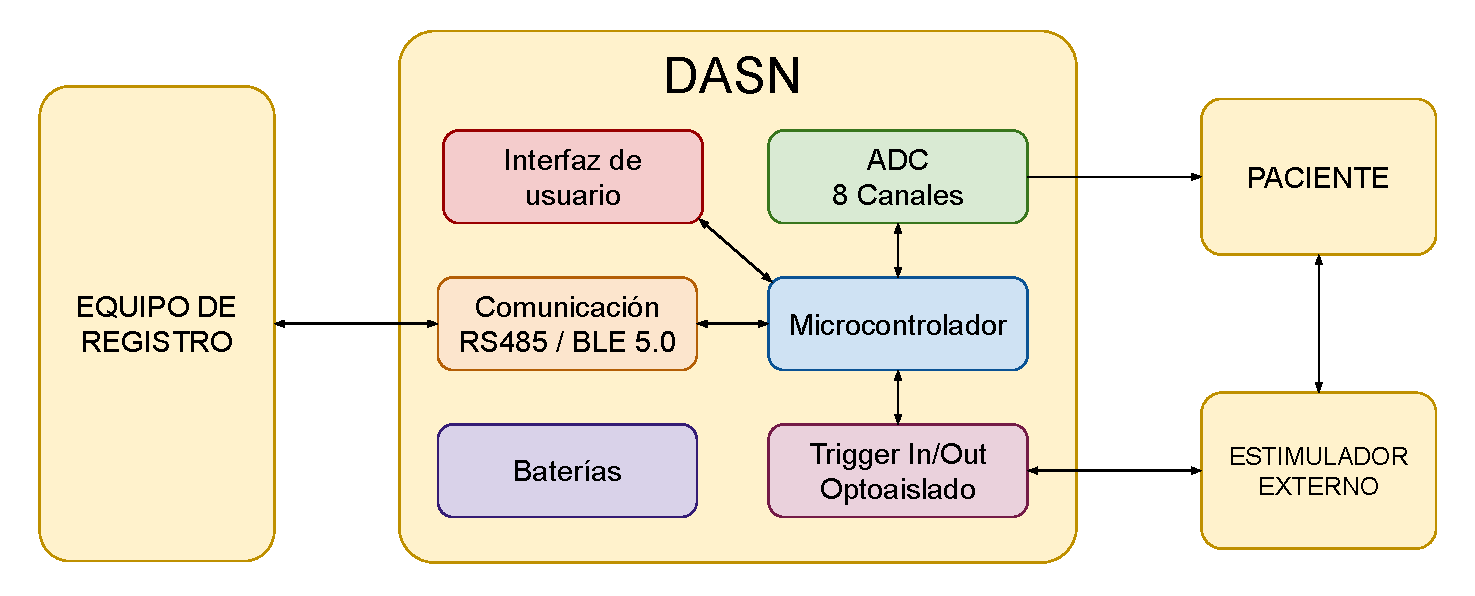
\includegraphics[width=0.94\textwidth]{./Figuras/DiagramaEnBloquesDASN.pdf}
\caption{Diagrama en bloques del sistema.}
\label{fig:diagBloquesSistema}
\end{figure}

El DASN tendrá 8 canales de entrada para adquirir las señales neurofisiológicas del paciente y las transmitirá al equipo de registro de manera inalámbrica a través de una comunicación BLE 5.0, o cableada a través de una comunicación RS485. Las señales adquiridas se podrán sincronizar con un estimulador externo, pudiendo funcionar el estimulador como master o slave. La interfaz de usuario solo dará indicaciones de encendido, apagado y estado de funcionamiento, ya que las señales adquiridas se visualizarán en el monitor del equipo de registro. El DASN se alimentará a baterías.

\section{2. Identificación y análisis de los interesados}
\label{sec:interesados}

\begin{table}[ht]
%\caption{Identificación de los interesados}
%\label{tab:interesados}
\begin{tabularx}{\linewidth}{@{}|l|X|X|l|@{}}
\hline
\rowcolor[HTML]{C0C0C0} 
Rol           & Nombre y Apellido & Organización 	& Puesto 	\\ \hline
%Auspiciante   & -		          &\pertesupname  	& -       	\\ \hline
Cliente       & \clientename      &\empclientename	& Director del proyecto     	\\ \hline
%Impulsor      &                   &              	&        	\\ \hline
Responsable   & \authorname       & FIUBA        	& Alumno 	\\ \hline
%Colaboradores &                   &              	&        	\\ \hline
%Orientador    & \supname	      & \pertesupname   & Director trabajo final \\ \hline
Orientador    & \cosupname	      & \pertecosupname   & Codirector trabajo final \\ \hline
%Equipo        & \authorname 	  & FIUBA         	& Alumno  	\\ \hline
%Opositores    &                   &              	&        	\\ \hline
%Usuario final &                   &              	&        	\\ \hline
\end{tabularx}
\end{table}

\begin{itemize}
	\item Dr. Ing. Diego Coulombie: Tiene experiencia en la redacción de documentos académicos. Puede ayudar en la elaboración de la memoria descriptiva final del proyecto.
	\item Ing. Ariel Gentile: Tiene experiencia en programación. Puede ayudar en el desarrollo de los módulos de software.
\end{itemize}

\section{3. Propósito del proyecto}
\label{sec:proposito}

El propósito de este proyecto es poner en práctica todos los conocimientos adquiridos durante la carrera de especialización, colaborar con el proyecto ''C2-ING-066 Herramientas de uso comunitario para el desarrollo de la industria de Tecnología Neurofisiológica", y a su vez, completar los requisitos de aprobación de la CESE.

\section{4. Alcance del proyecto}
\label{sec:alcance}

El presente proyecto incluye:
\begin{itemize}
	\item Diseño del firmware embebido del DASN.
	\item Diseño del protocolo de comunicación entre DASN y equipo de registro.
	\item Documentación acorde a norma ISO 62304.
	\item Software de prueba para simular un equipo de registro y probar el DASN.
\end{itemize}

El presente proyecto no incluye:
\begin{itemize}
	\item Diseño de hardware.
	\item Filtrado digital de las señales adquiridas.
	\item Validación de norma ISO 62304.
\end{itemize}


\section{5. Supuestos del proyecto}
\label{sec:supuestos}

Para el desarrollo del presente proyecto se supone que:
\begin{itemize}
	\item El cliente proveerá del hardware necesario para el desarrollo del firmware.
	\item El protocolo de comunicación entre el DASN y el equipo de registro es de libre diseño.
	\item El DASN y el equipo de registro estarán siempre cerca por lo que no hay requisitos de alcance en la comunicación inalámbrica.
	\item El hardware no cambiará durante el desarrollo del proyecto.
	\item La validación de la norma ISO 62304 en laboratorio acreditado queda a cargo del cliente.
\end{itemize}

\section{6. Requerimientos}
\label{sec:requerimientos}

\begin{enumerate}
	\item \textbf{Requerimientos de interfaces externas}
		\begin{enumerate}
			\item El software deberá comunicarse con el equipo de registro utilizando una interfaz BLE 5.0.
			\item El software deberá comunicarse con el equipo de registro utilizando una interfaz RS485. 
			\item El software deberá indicar mediante el led1 que está transmitiendo las señales adquiridas de forma inalámbrica o cableada. 
			\item El software deberá indicar mediante el led2 si está encendido o apagado. También deberá indicar con el mismo led2 si entra en el modo pairing BLE.
			\item El software deberá manejar una salida para sincronizar la adquisición con un estimulador externo (dispositivo externo como slave). La salida deberá poder configurarse entre normal bajo y normal alto. El pulso deberá poder configurarse entre 5 anchos de pulso diferentes (0,1 ms; 0,5 ms; 1 ms; 5 ms; 10 ms). 
			\item El software deberá manejar una entrada para sincronizar la adquisición con un estimulador externo (dispositivo externo como master). La detección deberá ser por flanco y se deberá poder configurar si el flanco es de subida o de bajada.
			\item El software deberá manejar el pulsador que servirá para encender el dispositivo y para realizar el pairing BLE.
			\item El software deberá generar la señal de impedancia para los canales de potenciales evocados.
			\item El software deberá medir el estado de las baterías con el ADC interno del MCU.
		\end{enumerate}
	\item \textbf{Requerimientos funcionales}
		\begin{enumerate}
			\item El software deberá configurar la frecuencia de muestreo de la señal adquirida entre 7 diferentes valores ( el ADC de ''EEG-FrontEnd\_v1.x.0.SchDoc” ofrece 65 Hz, 131 Hz, 262 Hz, 524 Hz, 1048 Hz, 2096 Hz y 4193 Hz).
			\item El software deberá poder adquirir de 1 a 8 canales simultáneos.
			\item Mediante comandos recibidos por BLE 5.0 o RS485 el software deberá poder iniciar y parar la adquisición.
			\item El software deberá configurar la ganancia de amplificación de cada canal entre 7 diferentes valores ( el ADC de ''EEG-FrontEnd\_v1.x.0.SchDoc” ofrece 1, 2, 4, 6, 8, 12 y 24).
			\item El software deberá configurar el ADC para usar una tipología de entrada diferencial o referencial.
			\item El software deberá medir la impedancia de los electrodos con una señal de medición de impedancia cuya frecuencia deberá ser de 7,8 Hz o 31,2 Hz.
			\item El software deberá seleccionar a qué electrodos le inyecta la señal de medición de impedancia.
			\item El software deberá seleccionar para cada electrodo si usa la señal de impedancia generada por el ADC o la generada por el MCU.
			\item El software deberá enviar la siguiente información de autodiagnóstico: temperatura del ADC, valor de las tensiones del ADC y frecuencia del clock del ADC.
			\item El software deberá prender y apagar el equipo con una pulsación corta del botón, pulsación menor a 1 segundo.
			\item El software deberá entrar en el modo de apareo de la comunicación BLE con una pulsación larga del botón, pulsación mayor a 4 segundos.
			\item Luego de 1 minuto de inactividad, el software deberá entrar a un modo de bajo consumo de energía. Para esto deberá apagar el ADC, el transceiver RS485 y la alimentación de todos los periféricos externos al MCU.
			\item El software deberá manejar una comunicación RS485 hasta 3 MBd.
			\item El software deberá poder recibir comandos mientras está transmitiendo las señales adquiridas.

		\end{enumerate}
	\item \textbf{Requerimientos de documentación}
		\begin{enumerate}
			\item La documentación debe cumplir los requisitos de la norma ISO 62304.
			\item Toda la documentación del proyecto se almacenará bajo un sistema de control de versiones GIT.
			\item Toda la documentación del código se realizará utilizando la herramienta Doxygen.
			\item Se deberá realizar un informe de avance del proyecto en el séptimo mes de trabajo
			\item Se deberá realizar la memoria técnica del trabajo final con la plantilla elaborada por la cátedra de gestión de proyecto.
		\end{enumerate}
%	\item \textbf{Requerimientos futuros}
%		\begin{enumerate}	
%			\item En el futuro se prevé diseñar un hardware con hasta 32 canales de adquisición.
			
%		\end{enumerate}
\end{enumerate}

\section{7. Historias de usuarios (\textit{Product backlog})}
\label{sec:backlog}

Criterio para ponderar los \textit{story points}: 

Se deben evaluar los siguientes aspectos de cada historia de usuario con una escala de 1 a 3, donde 1 es la calificación más baja y 3 la más alta:
\begin{itemize}
	\item \textbf{Dificultad} (cantidad de trabajo a realizar).
	\item \textbf{Complejidad} (nivel de sofisticación del trabajo).
	\item \textbf{Incertidumbre} (nivel de riesgo que involucra realizar la tarea).
\end{itemize}	

Finalmente se determinan los \textit{story points} realizando la siguiente operación:

\textbf{\textit{Story points}} = Dificultad x Complejidad x Incertidumbre


	\begin{enumerate}
		\item ''Como usuario quiero seleccionar la frecuencia de muestreo y ganancia de cada canal para poder hacer distintos tipos de estudios neurológicos."
		\begin{itemize}
			\item \textbf{Dificultad:} 1
			\item \textbf{Complejidad:} 2
			\item \textbf{Incertidumbre:} 1
		\end{itemize}	
	\textbf{\textit{Story points}} = 2

		\item ''Como usuario quiero que el equipo sea inalámbrico para que el paciente se mueva libremente"
		\begin{itemize}
			\item \textbf{Dificultad:} 2
			\item \textbf{Complejidad:} 3
			\item \textbf{Incertidumbre:} 3
		\end{itemize}	
	\textbf{\textit{Story points}} = 18

		\item ''Como usuario quiero medir la impedancia de los electrodos para poder comprobar su correcta colocación."
		\begin{itemize}
			\item \textbf{Dificultad:} 2
			\item \textbf{Complejidad:} 2
			\item \textbf{Incertidumbre:} 1
		\end{itemize}	
	\textbf{\textit{Story points}} = 4

		\item ''Como usuario quiero sincronizar el equipo con un estimulador externo para hacer estudios de potenciales evocados."
		\begin{itemize}
			\item \textbf{Dificultad:} 2
			\item \textbf{Complejidad:} 2
			\item \textbf{Incertidumbre:} 2
		\end{itemize}	
	\textbf{\textit{Story points}} = 8

		\item ''Como usuario quiero ver el estado de las baterías para saber la autonomía del equipo."
		\begin{itemize}
			\item \textbf{Dificultad:} 2
			\item \textbf{Complejidad:} 2
			\item \textbf{Incertidumbre:} 2
		\end{itemize}	
	\textbf{\textit{Story points}} = 8
	\end{enumerate}

%\begin{consigna}{red}
%Descripción: En esta sección se deben incluir las historias de usuarios y su ponderación (\textit{history points}). Recordar que las historias de usuarios son descripciones cortas y simples de una característica contada desde la perspectiva de la persona que desea la nueva capacidad, generalmente un usuario o cliente del sistema. La ponderación es un número entero que representa el tamaño de la historia comparada con otras historias de similar tipo.
%
%El formato propuesto es: "como [rol] quiero [tal cosa] para [tal otra cosa]."
%
%Se debe indicar explícitamente el criterio para calcular los \textit{story points} de cada historia
%\end{consigna}

\section{8. Entregables principales del proyecto}
\label{sec:entregables}

Los entregables del proyecto son:

\begin{itemize}
	\item Código fuente del firmware.
	\item Código fuente del Software de prueba.
	\item Documentación acorde a ISO 62304.
	\item Informe final.
\end{itemize}

\section{9. Desglose del trabajo en tareas}
\label{sec:wbs}

En cada grupo de tareas se indica el subtotal de horas correspondiente al mismo.

\begin{enumerate}
\item \textbf{Planificación y documentación (100 hs)}
	\begin{enumerate}
	\item Planificación del proyecto (20 hs)
	\item Especificación de requisitos de software (20 hs)
	\item Investigación Norma ISO 62304 (30 hs)
	\item Análisis de riesgo (30 hs)
	\end{enumerate}
\item \textbf{Diseño e implementación del firmware (270 hs)}
	\begin{enumerate}
	\item Preparación del entorno de desarrollo (20 hs)
	\item Diseño de la arquitectura del firmware  (30 hs)
	\item Investigación sobre tecnología BLE (20 hs)	
	\item Diseño del protocolo de comunicación (30 hs)
	\item Desarrollo del módulo comunicación BLE (40 hs)
	\item Desarrollo del módulo comunicación RS485 (20 hs)
	\item Desarrollo del módulo ADC (30 hs)
	\item Desarrollo del módulo manejo estimulador externo (20 hs)
	\item Desarrollo del módulo interfaz de usuario (10 hs)
	\item Pruebas de integración (30 hs)
	\item Pruebas de verificación (20 hs)
	\end{enumerate}
\item \textbf{Diseño e implementación software de prueba (150 hs)}
	\begin{enumerate}
	\item Preparación del entorno de desarrollo (20 hs)
	\item Diseño de la arquitectura (20 hs)
	\item Desarrollo de drivers (40 hs)
	\item Desarrollo de Interfaz gráfica (30 hs)
	\item Pruebas de integración (20 hs)
	\item Pruebas de verificación (20 hs)
	\end{enumerate}
\item \textbf{Cierre del proyecto (110 hs)}
	\begin{enumerate}
	\item Pruebas de validación (40 hs)
	\item Confección de informes de avance del proyecto (10 hs)
	\item Presentaciones al cliente (10 hs)
	\item Elaboración de la memoria descriptiva final del proyecto  (40 hs)
	\item Presentación final del proyecto (10 hs)
	\end{enumerate}
\end{enumerate}

\textbf{Cantidad total de horas: (630 hs)}

\newpage
\section{10. Diagrama de Activity On Node}
\label{sec:AoN}

\begin{figure}[htpb]
\centering 
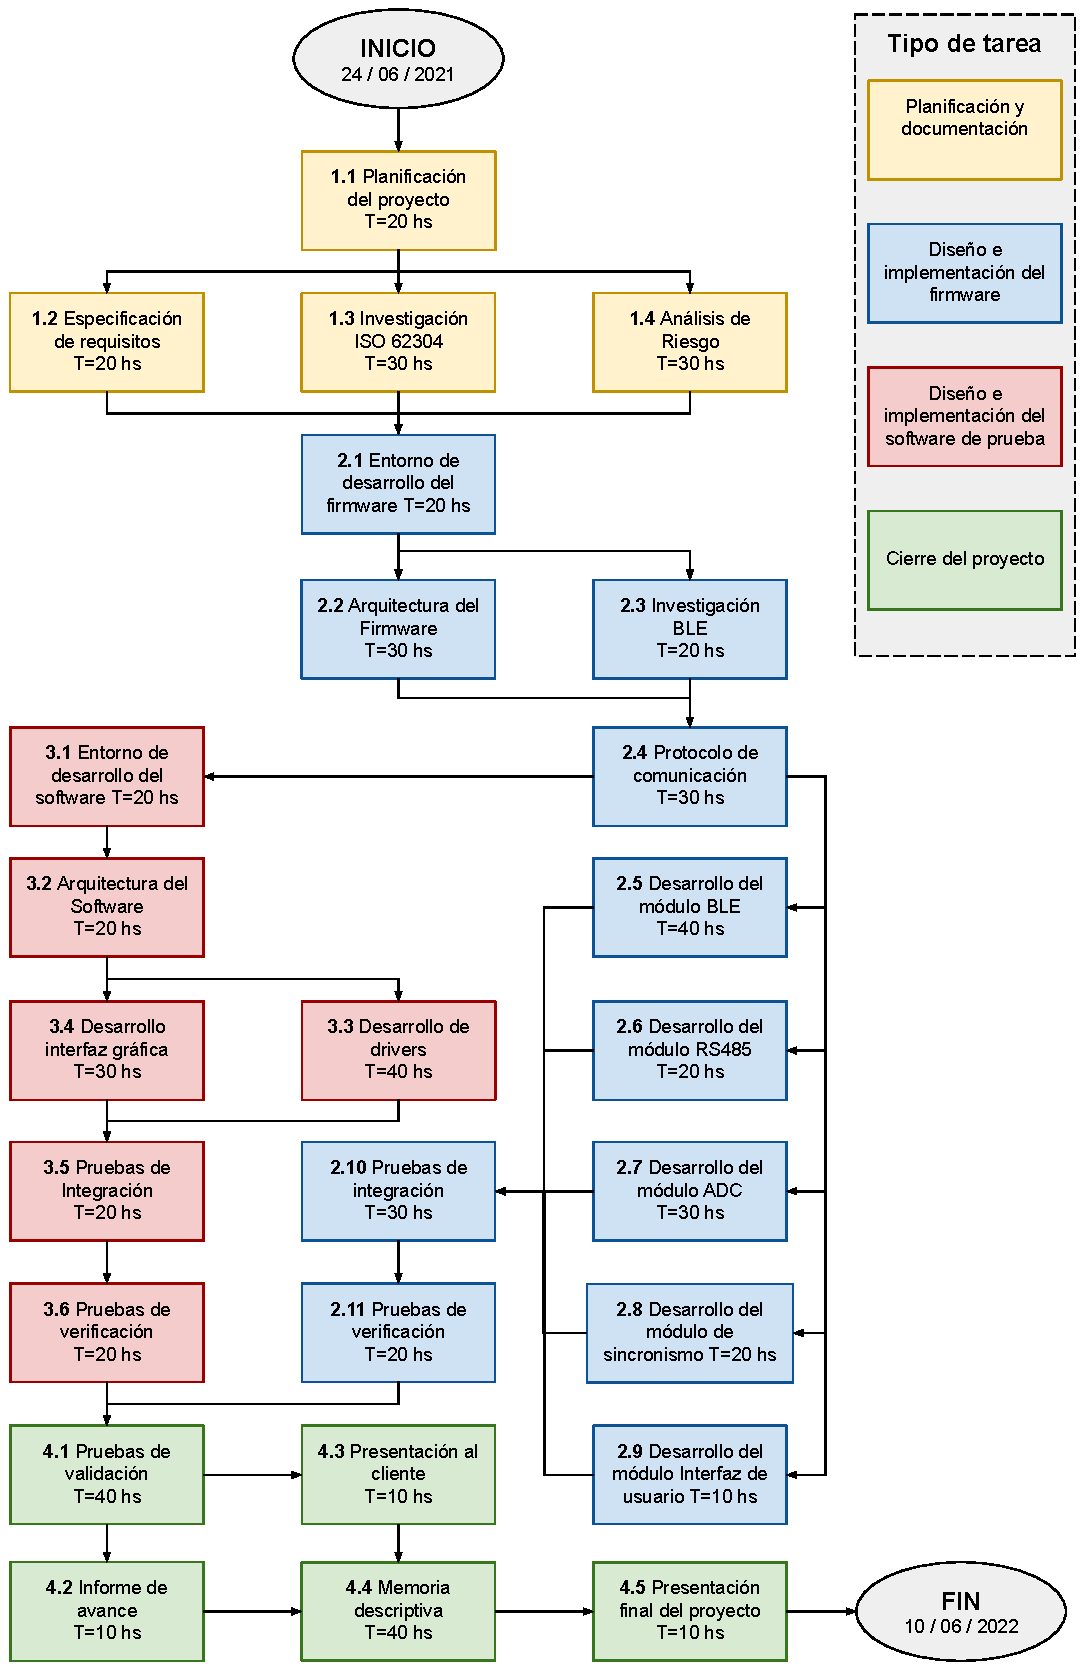
\includegraphics[width=0.75\textwidth]{./Figuras/DASNActivityonNode.pdf}
\caption{Diagrama de \textit{Activity on Node.}}
\label{fig:AoN}
\end{figure}

%\begin{landscape}

\section{11. Diagrama de Gantt}
\label{sec:gantt}

\begin{figure}[htpb]
\centering 
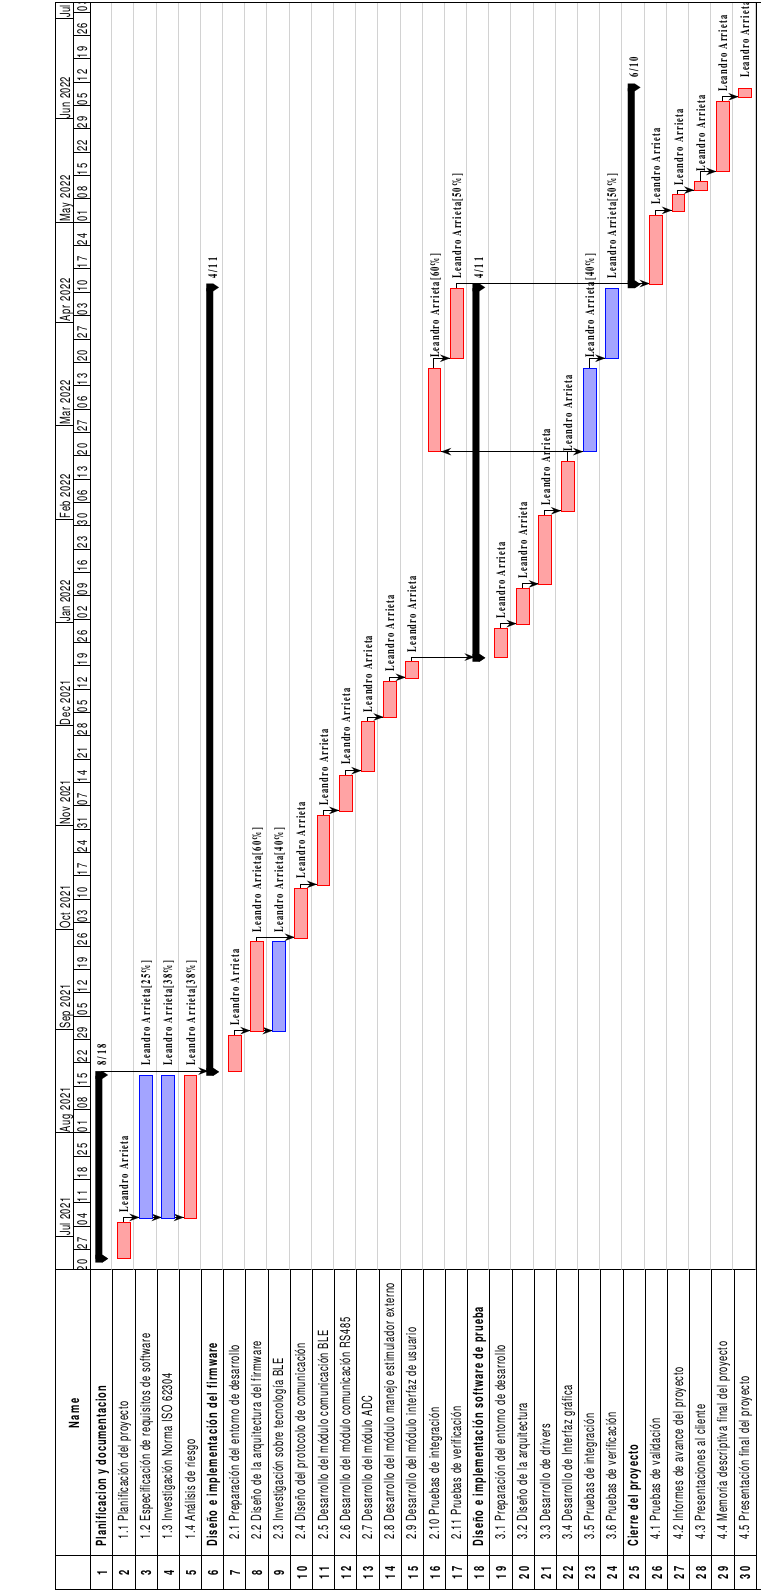
\includegraphics[height=.96\textheight]{./Figuras/DASNGantt.png}
\caption{Diagrama de Gantt}
\label{fig:diagGantt}
\end{figure}

%\end{landscape}


\section{12. Presupuesto detallado del proyecto}
\label{sec:presupuesto}

\begin{table}[htpb]
\centering
\begin{tabularx}{\linewidth}{@{}|X|c|r|r|@{}}
\hline
\rowcolor[HTML]{C0C0C0} 
\multicolumn{4}{|c|}{\cellcolor[HTML]{C0C0C0}COSTOS DIRECTOS} \\ \hline
\rowcolor[HTML]{C0C0C0} 
 Descripción & Cantidad & Valor unitario & Valor total \\ \hline

 Mano de obra & 630 & u\$s 10,00 & u\$s 6300,00 \\ \hline
 Módulo de desarrollo LAUNCHXL-CC2640R2 & 2 & u\$s 34,80 & u\$s 69,60 \\ \hline
 Módulo de desarrollo ADS1299EEGFE-PDK & 1 & u\$s 238,80 & u\$s 238,80 \\ \hline
\multicolumn{3}{|c|}{SUBTOTAL} & u\$s 6608,40 \\ \hline
\rowcolor[HTML]{C0C0C0} 
\multicolumn{4}{|c|}{\cellcolor[HTML]{C0C0C0}COSTOS INDIRECTOS} \\ \hline
\rowcolor[HTML]{C0C0C0} 
 Descripción & Cantidad & Valor unitario & Valor total \\ \hline

 Costos indirectos, estimados como 20\% de los los costos directos & 1 & u\$s 1321,68  & u\$s 1321,68  \\ \hline

\multicolumn{3}{|c|}{SUBTOTAL} & u\$s 1321,68 \\ \hline
\rowcolor[HTML]{C0C0C0}
\multicolumn{3}{|c|}{TOTAL} & u\$s 7930,08   \\ \hline
\end{tabularx}%
\end{table}


\section{13. Gestión de riesgos}
\label{sec:riesgos}

Criterio para ponderar los riesgos:
\begin{itemize}
	\item Severidad (S): Rango de 1 a 10. Mientras más severo, más alto es el número.
	\item Probabilidad de ocurrencia (O): Rango de 1 a 10. Mientras más probable, más alto es el número.
\end{itemize}

\textbf{a)} A continuación se listan los riesgos asociados al proyecto:

\begin{enumerate} 
	\item[] \textbf{Riesgo 1:} Retraso en la fecha de finalización del proyecto.
	\begin{itemize}
		\item \textbf{Severidad (10):} Implica incumplimiento con el cliente y la no aprobación de la CESE.
		\item \textbf{Ocurrencia (5):} El responsable del proyecto no posee experiencia en la programación de sistemas embebidos por lo que la ejecución de las tareas puede llevar más tiempo del planificado. 
	\end{itemize} 

	\item[] \textbf{Riesgo 2:} Errores en el diseño del hardware impiden probar el firmware.
	\begin{itemize}
		\item \textbf{Severidad (7):} La falta de prototipo demora las pruebas de validación.
		\item \textbf{Ocurrencia (7):} Quienes desarrollaron el hardware no tenían experiencia en el desarrollo de equipos con el MCU seleccionado ni con equipos inalámbricos.
	\end{itemize} 

	\item[] \textbf{Riesgo 3:} Daños en el prototipo de hardware durante el desarrollo.
	\begin{itemize}
		\item \textbf{Severidad (7):} La falta de prototipo demora las pruebas de validación.
		\item \textbf{Ocurrencia (2):} Existen 3 prototipos armados por lo que la probabilidad de quedarse sin prototipo para las pruebas es baja.
	\end{itemize} 

	\item[] \textbf{Riesgo 4:} No cumplir con todos los requerimientos.
	\begin{itemize}
		\item \textbf{Severidad (9):} El producto final no funcionará como se espera.
		\item \textbf{Ocurrencia (5):} El responsable del proyecto no posee experiencia en la programación de sistemas embebidos por lo que la ejecución de las tareas puede llevar más tiempo del planificado. 
	\end{itemize} 

	\item[] \textbf{Riesgo 5:} El rendimiento del hardware seleccionado no es suficiente para cumplir con todos los requisitos.
	\begin{itemize}
		\item \textbf{Severidad (9):} El producto final no funcionará como se espera. 
		\item \textbf{Ocurrencia (2):} Luego de analizar las hojas de datos de los principales componentes y ver los ejemplos de aplicación del fabricante se infiere una baja probabilidad de ocurrencia de este riesgo.
	\end{itemize}
\end{enumerate}

\textbf{b)} Tabla de gestión de riesgos: (El RPN se calcula como RPN = S x O)

\begin{table}[htpb]
\centering
\begin{tabular}{|c|c|c|c|c|c|c|}
\hline
\rowcolor[HTML]{C0C0C0} 
Riesgo & S & O & 			RPN			 		  & S* & O* & RPN* \\ \hline
1 & 10 & 5 & \textcolor{red}{50} & 10 & 3  &  \textcolor[HTML]{009900}{30} \\ \hline
2      & 7  & 7 & \textcolor{red}{49} & 5 & 5  &  \textcolor[HTML]{009900}{25} \\ \hline
3      & 7  & 2 & \textcolor[HTML]{009900}{14} &  &  & \\ \hline
4      & 9  & 5 & \textcolor{red}{45} & 9 & 3  &  \textcolor[HTML]{009900}{27} \\ \hline
5      & 9  & 2 & \textcolor{red}{18} &  &   & \\ \hline
\end{tabular}
\end{table}

Criterio adoptado: 
Se tomarán medidas de mitigación en los riesgos cuyos números de RPN sean mayores a 30.

Nota: los valores marcados con (*) en la tabla corresponden luego de haber aplicado la mitigación.

\textbf{c)} Plan de mitigación de los riesgos que originalmente excedían el RPN máximo establecido:

\begin{enumerate} 
	\item[] \textbf{Riesgo 1:} 
	
	\textbf{Plan de mitigación:} Se efectuará un seguimiento semanal del grado de avance de las tareas respecto a la planificación para detectar retrasos tempranos.
	\begin{itemize}
		\item \textbf{Severidad (10):} La severidad del riesgo no cambia con la medida adoptada.
		\item \textbf{Ocurrencia (3):} Al detectarse un retraso en forma temprana se pueden aumentar los esfuerzos para cumplir con la planificación.
	\end{itemize} 
	\item[] \textbf{Riesgo 2:} 

	\textbf{Plan de mitigación:} Se comprarán placas de desarrollo de los principales módulos.
	\begin{itemize}
		\item \textbf{Severidad (5):} Con las placas de desarrollo se pueden probar la mayoría de los requisitos.
		\item \textbf{Ocurrencia (5):} Al tener otra alternativa para probar el firmware la probabilidad de no poder probarlo baja.
	\end{itemize} 
	\item[] \textbf{Riesgo 4:} 
	
	\textbf{Plan de mitigación:} Se planifican las tareas mas complejas y que mayor incertidumbre dan al comienzo del proyecto para tener margen de acción ante problemas para su ejecución.
	\begin{itemize}
		\item \textbf{Severidad (9):} La severidad del riesgo no cambia con la medida adoptada.
		\item \textbf{Ocurrencia (3):} Al detectarse un retraso en forma temprana se pueden aumentar los esfuerzos para cumplir con la planificación.
	\end{itemize} 

\end{enumerate}



\section{14. Gestión de la calidad}
\label{sec:calidad}

\begin{enumerate}
	\item \textbf{Requerimientos de interfaces externas}
		\begin{enumerate}
			\item El software deberá comunicarse con el equipo de registro utilizando una interfaz BLE 5.0.
			
			\textbf{Verificación:} Se verificarán las librerías y módulos de software utilizados.
			
			\textbf{Validación:} Pruebas de sistema sobre el producto final.
			\item El software deberá comunicarse con el equipo de registro utilizando una interfaz RS485. 
			
			\textbf{Verificación:} Se verificarán las librerías y módulos de software utilizados.
			
			\textbf{Validación:} Pruebas de sistema sobre el producto final.
			\item El software deberá indicar mediante el led1 que está transmitiendo las señales adquiridas de forma inalámbrica o cableada. 
			
			\textbf{Verificación:} Pruebas unitarias y de integración sobre las funciones asociadas. Inspección visual. 
			
			\textbf{Validación:} Pruebas de sistema sobre el producto final.  Inspección visual.
			\item El software deberá indicar mediante el led2 si está encendido o apagado. También deberá indicar con el mismo led2 si entra en el modo pairing BLE.
			
			\textbf{Verificación:} Pruebas unitarias y de integración sobre las funciones asociadas. Inspección visual.
			
			\textbf{Validación:} Pruebas de sistema sobre el producto final. Inspección visual.
			\item El software deberá manejar una salida para sincronizar la adquisición con un estimulador externo (dispositivo externo como slave). La salida deberá poder configurarse entre normal bajo y normal alto. El pulso deberá poder configurarse entre 5 anchos de pulso diferentes (0,1 ms; 0,5 ms; 1 ms; 5 ms; 10 ms). 
			
			\textbf{Verificación:} Pruebas unitarias y de integración sobre las funciones asociadas. 			
			
			\textbf{Validación:}  Pruebas de sistema sobre el producto final. Medición con osciloscopio sobre el producto final.
			\item El software deberá manejar una entrada para sincronizar la adquisición con un estimulador externo (dispositivo externo como master). La detección deberá ser por flanco y se deberá poder configurar si el flanco es de subida o de bajada.
			
			\textbf{Verificación:} Pruebas unitarias y de integración sobre las funciones asociadas. 			
			
			\textbf{Validación:}  Pruebas de sistema sobre el producto final. Se inyectará un pulso de sincronismo sobre el producto final.
			\item El software deberá manejar el pulsador que servirá para encender el dispositivo y para realizar el pairing BLE.
			
			\textbf{Verificación:} Pruebas unitarias y de integración sobre las funciones asociadas. 
			
			\textbf{Validación:} Pruebas de sistema sobre el producto final. Se probará el funcionamiento del pulsador.
			\item El software deberá generar la señal de impedancia para los canales de potenciales evocados.
			
			\textbf{Verificación:} Se medirá con osciloscopio la señal de impedancia.
			
			\textbf{Validación:} Pruebas de sistema sobre el producto final. Se colocarán resistencias en los electrodos para medir la impedancia.
			\item El software deberá medir el estado de las baterías con el ADC interno del MCU.
			
			\textbf{Verificación:} Se conectará una fuente de tensión variable par verificar la medición de tensión de las baterías.
			
			\textbf{Validación:} Pruebas de sistema sobre el producto final. Se leerá la indicación del software y se contrastará midiendo las baterías con un multímetro.
		\end{enumerate}
	\item \textbf{Requerimientos funcionales}
		\begin{enumerate}
			\item El software deberá configurar la frecuencia de muestreo de la señal adquirida entre 7 diferentes valores ( el ADC de ''EEG-FrontEnd\_v1.x.0.SchDoc” ofrece 65 Hz, 131 Hz, 262 Hz, 524 Hz, 1048 Hz, 2096 Hz y 4193 Hz).
			
			\textbf{Verificación:} Pruebas unitarias y de integración sobre las funciones asociadas.
			
			\textbf{Validación:} Pruebas de sistema sobre el producto final. Se revisarán los archivos adquiridos por el producto final.
			\item El software deberá poder adquirir de 1 a 8 canales simultáneos.
			
			\textbf{Verificación:} Pruebas unitarias y de integración sobre las funciones asociadas.
			
			\textbf{Validación:} Pruebas de sistema sobre el producto final. Inspección visual en el dispositivo de registro.
			\item Mediante comandos recibidos por BLE 5.0 o RS485 el software deberá poder iniciar y parar la adquisición.
			
			\textbf{Verificación:} Pruebas unitarias y de integración sobre las funciones asociadas.
			
			\textbf{Validación:} Pruebas de sistema sobre el producto final. Inspección visual en el dispositivo de registro.
			\item El software deberá configurar la ganancia de amplificación de cada canal entre 7 diferentes valores ( el ADC de ''EEG-FrontEnd\_v1.x.0.SchDoc” ofrece 1, 2, 4, 6, 8, 12 y 24).
			
			\textbf{Verificación:} Pruebas unitarias y de integración sobre las funciones asociadas.
			
			\textbf{Validación:} Pruebas de sistema sobre el producto final.
			\item El software deberá configurar el ADC para usar una tipología de entrada diferencial o referencial.
			
			\textbf{Verificación:} Pruebas unitarias y de integración sobre las funciones asociadas.
			
			\textbf{Validación:} Pruebas de sistema sobre el producto final. Se inyectará señal en las entradas según configuración seleccionada.
			\item El software deberá medir la impedancia de los electrodos con una señal de medición de impedancia cuya frecuencia deberá ser de 7,8 Hz o 31,2 Hz.
			
			\textbf{Verificación:} Se medirá con osciloscopio la señal de medición de impedancia.
			
			\textbf{Validación:} Pruebas de sistema sobre el producto final.
			\item El software deberá seleccionar a qué electrodos le inyecta la señal de medición de impedancia.
			
			\textbf{Verificación:} Pruebas unitarias y de integración sobre las funciones asociadas. Se medirá con osciloscopio la señal de medición de impedancia.
			
			\textbf{Validación:} Pruebas de sistema sobre el producto final. Inspección visual en el dispositivo de registro.
			\item El software deberá seleccionar para cada electrodo si usa la señal de impedancia generada por el ADC o la generada por el MCU.
			
			\textbf{Verificación:} Pruebas unitarias y de integración sobre las funciones asociadas. Se medirá con osciloscopio la señal de medición de impedancia.
			
			\textbf{Validación:}  Pruebas de sistema sobre el producto final. Se colocarán resistencias en los electrodos para medir la impedancia.
			\item El software deberá enviar la siguiente información de autodiagnóstico: temperatura del ADC, valor de las tensiones del ADC y frecuencia del clock del ADC.
			
			\textbf{Verificación:} Pruebas unitarias y de integración sobre las funciones asociadas.
			
			\textbf{Validación:}  Pruebas de sistema sobre el producto final.
			\item El software deberá prender y apagar el equipo con una pulsación corta del botón, pulsación menor a 1 segundo.
			
			\textbf{Verificación:} Pruebas unitarias y de integración sobre las funciones asociadas.
			
			\textbf{Validación:} Pruebas de sistema sobre el producto final. Se probará el funcionamiento del botón.
			\item El software deberá entrar en el modo de apareo de la comunicación BLE con una pulsación larga del botón, pulsación mayor a 4 segundos.
			
			\textbf{Verificación:} Pruebas unitarias y de integración sobre las funciones asociadas.
			
			\textbf{Validación:} Pruebas de sistema sobre el producto final. Se probará el funcionamiento del botón.
			\item Luego de 1 minuto de inactividad, el software deberá entrar a un modo de bajo consumo de energía. Para esto deberá apagar el ADC, el transceiver RS485 y la alimentación de todos los periféricos externos al MCU.
			
			\textbf{Verificación:} Pruebas unitarias y de integración sobre las funciones asociadas.
			
			\textbf{Validación:} Pruebas de sistema sobre el producto final. Medición del consumo.
			\item El software deberá manejar una comunicación RS485 hasta 3 MBd.
			
			\textbf{Verificación:} Pruebas unitarias y de integración sobre las funciones asociadas.
			
			\textbf{Validación:} Pruebas de sistema sobre el producto final. Se probará la comunicación a 3MBd.
			\item El software deberá poder recibir comandos mientras está transmitiendo las señales adquiridas.
			
			\textbf{Verificación:} Pruebas unitarias y de integración sobre las funciones asociadas.
			
			\textbf{Validación:} Pruebas de sistema sobre el producto final. Se enviarán comandos mientras se adquiere señal. 

		\end{enumerate}
	\item \textbf{Requerimientos de documentación}
		\begin{enumerate}
			\item La documentación debe cumplir los requisitos de la norma ISO 62304.
			
			\textbf{Verificación:} Por inspección, se completará un checklist.
			
			\textbf{Validación:} No esta dentro de los alcances del proyecto.
			\item Toda la documentación del proyecto se almacenará bajo un sistema de control de versiones GIT. 
			
			\textbf{Verificación:} Por inspección del repositorio.
			
			\textbf{Validación:} Por inspección del repositorio.
			\item Toda la documentación del código se realizará utilizando la herramienta Doxygen.
			
			\textbf{Verificación:} Por inspección del código fuente.
			
			\textbf{Validación:} Por inspección de la página web generada.
			\item Se deberá realizar un informe de avance del proyecto en el séptimo mes de trabajo
			
			\textbf{Verificación:} Por inspección del informe.
			
			\textbf{Validación:} Por inspección del informe.
			\item Se deberá realizar la memoria técnica del trabajo final con la plantilla elaborada por la cátedra de gestión de proyecto.
					
			\textbf{Verificación:} Por inspección de la memoria.
			
			\textbf{Validación:} Por inspección de la memoria.
	\end{enumerate}

\end{enumerate}


\section{15. Procesos de cierre}    
\label{sec:cierre}


Al finalizar el proyecto se realizarán las siguientes actividades:
\begin{enumerate}
	\item Informe de evaluación final del proyecto, para lo cual se analizarán los siguientes aspectos:
		\begin{itemize}
			\item Si se cumplió con la fecha de finalización del proyecto.
			\item Si se tuvieron que utilizar más o menos recursos de los planificados para cumplir con el plan.
			\item Si se pudo cumplir con todos los requisitos planificados.
			\item Si se debieron tomar acciones no planificadas.
			\item Si aparecieron riesgos no contemplados originalmente.
			\item Si surgieron problemas y como se solucionaron.
			\item Nivel de satisfacción del cliente.
		\end{itemize}
	\item Transferencia de los entregables al cliente.
		\begin{itemize}
			\item Se coordinará una reunión con el cliente para tal fin.
		\end{itemize}
	\item Presentación pública en el marco de la CESE.

	\item Acto de cierre.
		\begin{itemize}
			\item Se realizará un acto de cierre con el objetivo de agradecer a todas las personas involucradas en el proyecto, miembros del jurado, docentes y autoridades de la CESE.
		\end{itemize}

\end{enumerate}


Todas las actividades del proceso de cierre estarán a cargo del responsable del proyecto.


\end{document}
